% Template adapted from the Eurographics SGP 2016 template
\documentclass{6838publ}
\usepackage{6838}
% \input{\string~/.macros}

\SpecialIssuePaper
\electronicVersion 
\ifpdf \usepackage[pdftex]{graphicx} \pdfcompresslevel=9
\else \usepackage[dvips]{graphicx} \fi
\graphicspath{{./assets}}


 
\PrintedOrElectronic

\usepackage{t1enc,dfadobe}
\usepackage{egweblnk}
\usepackage{cite}
\usepackage{lipsum}
\usepackage{amsmath}
\usepackage{amsfonts}
\usepackage{amssymb}

\newcommand\sa{\ensuremath{\mathcal{a}}}
\newcommand\sd{\ensuremath{\mathcal{d}}}
\newcommand\se{\ensuremath{\mathcal{e}}}
\newcommand\sg{\ensuremath{\mathcal{g}}}
\newcommand\sh{\ensuremath{\mathcal{h}}}
\newcommand\si{\ensuremath{\mathcal{i}}}
\newcommand\sj{\ensuremath{\mathcal{j}}}
\newcommand\sk{\ensuremath{\mathcal{k}}}
\newcommand\sm{\ensuremath{\mathcal{m}}}
\newcommand\sn{\ensuremath{\mathcal{n}}}
\newcommand\so{\ensuremath{\mathcal{o}}}
\newcommand\sq{\ensuremath{\mathcal{q}}}
\newcommand\sr{\ensuremath{\mathcal{r}}}
\newcommand\st{\ensuremath{\mathcal{t}}}
\newcommand\su{\ensuremath{\mathcal{u}}}
\newcommand\sv{\ensuremath{\mathcal{v}}}
\newcommand\sw{\ensuremath{\mathcal{w}}}
\newcommand\sx{\ensuremath{\mathcal{x}}}
\newcommand\sy{\ensuremath{\mathcal{y}}}
\newcommand\sz{\ensuremath{\mathcal{z}}}
\newcommand\sA{\ensuremath{\mathcal{A}}}
\newcommand\sB{\ensuremath{\mathcal{B}}}
\newcommand\sC{\ensuremath{\mathcal{C}}}
\newcommand\sD{\ensuremath{\mathcal{D}}}
\newcommand\sE{\ensuremath{\mathcal{E}}}
\newcommand\sF{\ensuremath{\mathcal{F}}}
\newcommand\sG{\ensuremath{\mathcal{G}}}
\newcommand\sH{\ensuremath{\mathcal{H}}}
\newcommand\sI{\ensuremath{\mathcal{I}}}
\newcommand\sJ{\ensuremath{\mathcal{J}}}
\newcommand\sK{\ensuremath{\mathcal{K}}}
\newcommand\sL{\ensuremath{\mathcal{L}}}
\newcommand\sM{\ensuremath{\mathcal{M}}}
\newcommand\sN{\ensuremath{\mathcal{N}}}
\newcommand\sO{\ensuremath{\mathcal{O}}}
\newcommand\sP{\ensuremath{\mathcal{P}}}
\newcommand\sQ{\ensuremath{\mathcal{Q}}}
\newcommand\sR{\ensuremath{\mathcal{R}}}
\newcommand\sS{\ensuremath{\mathcal{S}}}
\newcommand\sT{\ensuremath{\mathcal{T}}}
\newcommand\sU{\ensuremath{\mathcal{U}}}
\newcommand\sV{\ensuremath{\mathcal{V}}}
\newcommand\sW{\ensuremath{\mathcal{W}}}
\newcommand\sX{\ensuremath{\mathcal{X}}}
\newcommand\sY{\ensuremath{\mathcal{Y}}}
\newcommand\sZ{\ensuremath{\mathcal{Z}}}

\newcommand\ba{\ensuremath{\mathbf{a}}}
\newcommand\bb{\ensuremath{\mathbf{b}}}
\newcommand\bc{\ensuremath{\mathbf{c}}}
\newcommand\bd{\ensuremath{\mathbf{d}}}
\newcommand\be{\ensuremath{\mathbf{e}}}
\newcommand\bg{\ensuremath{\mathbf{g}}}
\newcommand\bh{\ensuremath{\mathbf{h}}}
\newcommand\bi{\ensuremath{\mathbf{i}}}
\newcommand\bj{\ensuremath{\mathbf{j}}}
\newcommand\bk{\ensuremath{\mathbf{k}}}
\newcommand\bl{\ensuremath{\mathbf{l}}}
\newcommand\bn{\ensuremath{\mathbf{n}}}
\newcommand\bo{\ensuremath{\mathbf{o}}}
\newcommand\bp{\ensuremath{\mathbf{p}}}
\newcommand\bq{\ensuremath{\mathbf{q}}}
\newcommand\br{\ensuremath{\mathbf{r}}}
\newcommand\bs{\ensuremath{\mathbf{s}}}
\newcommand\bt{\ensuremath{\mathbf{t}}}
\newcommand\bu{\ensuremath{\mathbf{u}}}
\newcommand\bv{\ensuremath{\mathbf{v}}}
\newcommand\bw{\ensuremath{\mathbf{w}}}
\newcommand\bx{\ensuremath{\mathbf{x}}}
\newcommand\by{\ensuremath{\mathbf{y}}}
\newcommand\bz{\ensuremath{\mathbf{z}}}
\newcommand\bA{\ensuremath{\mathbf{A}}}
\newcommand\bB{\ensuremath{\mathbf{B}}}
\newcommand\bC{\ensuremath{\mathbf{C}}}
\newcommand\bD{\ensuremath{\mathbf{D}}}
\newcommand\bE{\ensuremath{\mathbf{E}}}
\newcommand\bF{\ensuremath{\mathbf{F}}}
\newcommand\bG{\ensuremath{\mathbf{G}}}
\newcommand\bH{\ensuremath{\mathbf{H}}}
\newcommand\bI{\ensuremath{\mathbf{I}}}
\newcommand\bJ{\ensuremath{\mathbf{J}}}
\newcommand\bK{\ensuremath{\mathbf{K}}}
\newcommand\bL{\ensuremath{\mathbf{L}}}
\newcommand\bM{\ensuremath{\mathbf{M}}}
\newcommand\bN{\ensuremath{\mathbf{N}}}
\newcommand\bO{\ensuremath{\mathbf{O}}}
\newcommand\bP{\ensuremath{\mathbf{P}}}
\newcommand\bQ{\ensuremath{\mathbf{Q}}}
\newcommand\bR{\ensuremath{\mathbf{R}}}
\newcommand\bS{\ensuremath{\mathbf{S}}}
\newcommand\bT{\ensuremath{\mathbf{T}}}
\newcommand\bU{\ensuremath{\mathbf{U}}}
\newcommand\bV{\ensuremath{\mathbf{V}}}
\newcommand\bW{\ensuremath{\mathbf{W}}}
\newcommand\bX{\ensuremath{\mathbf{X}}}
\newcommand\bY{\ensuremath{\mathbf{Y}}}
\newcommand\bZ{\ensuremath{\mathbf{Z}}}
\newcommand\Ba{\ensuremath{\mathbb{a}}}
\newcommand\Bb{\ensuremath{\mathbb{b}}}
\newcommand\Bc{\ensuremath{\mathbb{c}}}
\newcommand\Bd{\ensuremath{\mathbb{d}}}
\newcommand\Be{\ensuremath{\mathbb{e}}}
\newcommand\Bf{\ensuremath{\mathbb{f}}}
\newcommand\Bg{\ensuremath{\mathbb{g}}}
\newcommand\Bh{\ensuremath{\mathbb{h}}}
\newcommand\Bi{\ensuremath{\mathbb{i}}}
\newcommand\Bj{\ensuremath{\mathbb{j}}}
\newcommand\Bk{\ensuremath{\mathbb{k}}}
\newcommand\Bl{\ensuremath{\mathbb{l}}}
\newcommand\Bm{\ensuremath{\mathbb{m}}}
\newcommand\Bn{\ensuremath{\mathbb{n}}}
\newcommand\Bo{\ensuremath{\mathbb{o}}}
\newcommand\Bp{\ensuremath{\mathbb{p}}}
\newcommand\Bq{\ensuremath{\mathbb{q}}}
\newcommand\Br{\ensuremath{\mathbb{r}}}
\newcommand\Bs{\ensuremath{\mathbb{s}}}
\newcommand\Bt{\ensuremath{\mathbb{t}}}
\newcommand\Bu{\ensuremath{\mathbb{u}}}
\newcommand\Bv{\ensuremath{\mathbb{v}}}
\newcommand\Bw{\ensuremath{\mathbb{w}}}
\newcommand\Bx{\ensuremath{\mathbb{x}}}
\newcommand\By{\ensuremath{\mathbb{y}}}
\newcommand\Bz{\ensuremath{\mathbb{z}}}
\newcommand\BA{\ensuremath{\mathbb{A}}}
\newcommand\BB{\ensuremath{\mathbb{B}}}
\newcommand\BC{\ensuremath{\mathbb{C}}}
\newcommand\BD{\ensuremath{\mathbb{D}}}
\newcommand\BE{\ensuremath{\mathbb{E}}}
\newcommand\BF{\ensuremath{\mathbb{F}}}
\newcommand\BG{\ensuremath{\mathbb{G}}}
\newcommand\BH{\ensuremath{\mathbb{H}}}
\newcommand\BI{\ensuremath{\mathbb{I}}}
\newcommand\BJ{\ensuremath{\mathbb{J}}}
\newcommand\BK{\ensuremath{\mathbb{K}}}
\newcommand\BL{\ensuremath{\mathbb{L}}}
\newcommand\BM{\ensuremath{\mathbb{M}}}
\newcommand\BN{\ensuremath{\mathbb{N}}}
\newcommand\BO{\ensuremath{\mathbb{O}}}
\newcommand\BP{\ensuremath{\mathbb{P}}}
\newcommand\BQ{\ensuremath{\mathbb{Q}}}
\newcommand\BR{\ensuremath{\mathbb{R}}}
\newcommand\BS{\ensuremath{\mathbb{S}}}
\newcommand\BT{\ensuremath{\mathbb{T}}}
\newcommand\BU{\ensuremath{\mathbb{U}}}
\newcommand\BV{\ensuremath{\mathbb{V}}}
\newcommand\BW{\ensuremath{\mathbb{W}}}
\newcommand\BX{\ensuremath{\mathbb{X}}}
\newcommand\BY{\ensuremath{\mathbb{Y}}}
\newcommand\BZ{\ensuremath{\mathbb{Z}}}
\newcommand\balpha{\ensuremath{\mbox{\boldmath$\alpha$}}}
\newcommand\bbeta{\ensuremath{\mbox{\boldmath$\beta$}}}
\newcommand\btheta{\ensuremath{\mbox{\boldmath$\theta$}}}
\newcommand\bphi{\ensuremath{\mbox{\boldmath$\phi$}}}
\newcommand\bpi{\ensuremath{\mbox{\boldmath$\pi$}}}
\newcommand\bpsi{\ensuremath{\mbox{\boldmath$\psi$}}}
\newcommand\bmu{\ensuremath{\mbox{\boldmath$\mu$}}}

\newcommand\R{\ensuremath{\mathbb{R}}} % Real numbers
\newcommand\Z{\ensuremath{\mathbb{Z}}} % Integers


\newcommand{\norm}[1]{\left\lVert#1\right\rVert}
\newcommand\inner[2]{\ensuremath{\left< #1, #2 \right>}} % Inner product
\DeclareMathOperator*{\diag}{diag} % Diagonal matrix
\newcommand\p[1]{\ensuremath{\left( #1 \right)}} % Parenthesis ()
\newcommand\pa[1]{\ensuremath{\left\langle #1 \right\rangle}} % <>
\newcommand\pb[1]{\ensuremath{\left[ #1 \right]}} % []
\newcommand\pc[1]{\ensuremath{\left\{ #1 \right\}}} % {}
\DeclareMathOperator*{\tr}{tr}


\title[]{Optimal Transport based Probabilistic Diffeomorphic Registration}

\author[P.W.]
       {Peiqi Wang
        \\
        MIT Department of Electrical Engineering and Computer Science\\
       }

\begin{document}

\teaser{
 \includegraphics[width=.9\linewidth]{{assets/amoeba0/plt_lddmm_points}}
 \centering
  \caption{The red amoeba is registered to blue amoeba. A valid diffeomorphic transformation can be generated from per-particle momenta (orange arrow) by solving a set of Geodesic equations (black dashed line). On the right, we can visualize variance of the effect of random transformation on shape as a heatmap. Although the two shapes is matched almost perfectly, the two legs flips over itself respectively and we are able to spot this mistake from the uncertainty heatmap.}
\label{fig:teaser}
}

\maketitle

\begin{abstract}
    In this project, we implemented optimal transport based diffeomorphic registration algorithms. We extended the current algorithm to account for uncertainty in the transformation mapping, and showed that such extension is useful for identifying errors.
\end{abstract}

\section{Introduction}

% narrow in no topic: remind this is a graphics paper, need to help them to figure out what topic and area of research. no need to wax poetic about topic's importance


% dig a hole: convince reader there is a problem with the state of the world. prior work may exist but its missing something important or there is a missing opportunity. the reading should be drooling for a bright future just out of reach

Diffeomorphic registration of shapes with unknown correspondence is an important step in medical data processing. The choice of similarity metric for good matching distinguishes the different algorithms in this domain. Recent work explored the use of entropic regularized wasserstein distance as a global measure of similarity between encoding of shapes as discrete measures \cite{feydyOptimalTransportDiffeomorphic2017a,feydyFastScalableOptimal2019}. However, a point estimate of the transformation yield errors that may invalidate downstream processing pipelines or misguide clinical decision making. Additionally, solution is sensitive to hyperparameters of the problem, requiring manual tuning for each new shape. 

% fill the hole: to show reader how/why the paper will fix these problems and deliver us into a better place. don't need a whirlwind summary of technical details, but need reader's convinced to keep reading. 

We propose to extend optimal transport based diffeomorphic registration to probabilistic setting. Our method interprets the diffeomorphic transformation as a random variable, and estimates its parameters using variational inference. In particular, we find diffeomorphic maps that minimize the average optimal transport distance between shapes. Naturally, the probabilistic formulation provides us with uncertainty estimates of both the transformation as well as the uncertainty of its effect on shapes. Hyperparameters such as the degree of smoothness of the transformation parameterizes the variational distribution, and thus can be optimized. 


% However, the inference procedure requires repeated sampling of valid diffeomorphic transformations to approximate the average cost. To alleviate the computational burden, we explored links to sparse Gaussian Process, specifically interdomain inducing variables, as a way to alleviate this concern \cite{figueiras-vidalInterdomainGaussianProcesses2009a}.


\section{Related Work}

\subsection{Diffeomorphic Registration}

The large deformation registration of landmarks (point sets) and images as a variational problem that solves for a smooth time-varying velocity field that matches the two objects according to some measure of similarity \cite{joshiLandmarkMatchingLarge2000,begComputingLargeDeformation2005}. \cite{millerGeodesicShootingComputational2006,vialardDiffeomorphic3DImage2012} makes connection to optimal control, and showed that large deformation diffeormorphisms obeys conservation of momentum, and that points/images evolve according to a set of Geodesic Equations completely determined by its initial momentum. This observation prompted the development of geodesic shooting methods that optimizes for initial momentum for point sets and meshes \cite{vaillantStatisticsDiffeomorphismsTangent2004,allassonniereGeodesicShootingDiffeomorphic2005} and later extended to images \cite{vialardDiffeomorphic3DImage2012}. In our formulation, we represent a random diffeomorphic map as a pushforward of initial momentum, parameterized by some easy-to-work-with distribution.

\subsection{Optimal Transport}

The optimal transport problem give rise to a notion of distance between probability distributions. Intuitively, it measures the amount of mass needed to be displaced from one measure to another. Computation of such distance is useful in numerous graphics \cite{degoesOptimalTransportApproach2011,degoesBlueNoiseOptimal2012,solomonConvolutionalWassersteinDistances2015} and learning \cite{frognerLearningWassersteinLoss2015, janatiSpatioTemporalAlignmentsOptimal2020} applications. Developments in numerical methods in computing and differentiating through the optimal transport distance make for easier integration to a larger system \cite{cuturiSinkhornDistancesLightspeed2013,altschulerNearlinearTimeApproximation2018,genevayLearningGenerativeModels2018,schmitzerStabilizedSparseScaling2019}. A series of work \cite{feydyOptimalTransportDiffeomorphic2017a,feydyFastScalableOptimal2019} utilize unbalanced optimal transport distance to register shapes with possibly different mass. The motivation is to combine the elastic properties of diffeomorphic registration beneficial for medical data with a cost that is sensitive to both local and global shape features. We extend their methods to probabilistic settings.


\subsection{Probabilistic Registration}

Many probabilistic registration methods on image data rely on latent variable model, where an unknown transformation is applied to the source image to generate the target image, corrupted by some observation noise. Previously, Monte Carlo methods have been used to estimate transformation parameters \cite{risholmBayesianCharacterizationUncertainty2013,zhangBayesianEstimationRegularization2013}. Although asymptotically exact, sampling methods can be slow for estimating the high dimensional parameters of a diffeomorphism. A few follow ups suggests ways to reduce the number of parameters using factor analysis \cite{risholmBayesianCharacterizationUncertainty2013} or with an economical representation in the Fourier domain \cite{wangRegistrationUncertaintyQuantification2019}. Alternatively, variational inference has been proposed as a more tractable alternative for inference \cite{wassermannProbabilisticDiffeomorphicRegistration2014,dalcaUnsupervisedLearningProbabilistic2019}. Although similar in formulation, we differ from \cite{wassermannProbabilisticDiffeomorphicRegistration2014} as we restrict ourselves to diffeomorphic registration of discrete representation of shapes with unknown correspondence. Theory from geodesic shooting implies that we do not need to model the Eulerian flow as the solution to some stochastic differential equation as proposed in \cite{wassermannProbabilisticDiffeomorphicRegistration2014}. It suffices to model the initial momentum as some Gaussian Process whereby to specify a random diffeomorphic transformations.

% Descriptions of and citations to academic research papers and/or existing software products related to your work.  Here is an example of how to cite a paper~\cite{solomon-2016}; see \texttt{6838bibsample.bib} for bibliography entries.


\section{Preliminaries}\label{sec:preliminaries}


\subsection{Shape as Measures}

Let $\Omega \subset\R^D$ be a low dimensional ambient space. We consider a representation of shapes as discrete measures $\alpha = \sum_{i=1}^N a_i \delta_{x_i}, \beta = \sum_{j=1}^M b_i \delta_{y_j}$ where $a_i,b_j\in\R_+$ encodes some local statistics of shape, e.g. per-vertex length for curves or per-vertex area for surfaces, and $x := (x^1,\cdots,x^n)\subset \R^{N\times D}$, $y := (y^1,\cdots,y^n)\subset\R^{M\times D}$ are source and target points respectively. 


\subsection{Diffeomorphic Registration}
% We follow the usual setup for registering unlabeled point sets using geodesic shooting \cite{vaillantStatisticsDiffeomorphismsTangent2004}. 


The goal of diffeomorphic registration of point sets is to transform $x$ via a diffeomorphic mapping $\varphi$ such that the pushforward $\varphi_\sharp \alpha$ is close to $y$ according to some similarity metric $\sL(\varphi_\sharp \alpha, \beta)$. We consider a space of velocity fields $V$ as a RKHS over $\Omega$ characterized by kernel $\overline{k}:\Omega\times\Omega\to\R^{D\times D}$. For purposes of computation, we consider an equivalent scalar-valued kernel $k:\Omega\times[D]\times\Omega\times[D] \to\R$ where $\overline{k}(x,x')_{dd'} = k((x,d),(x',d'))$, inducing an RKHS that is isomorphic to $V$. A diffeomorphism can be constructed via flows, i.e. solutions to an ODE problem $\varphi_t$ where $\dot{\varphi}_t = v_t\circ \varphi_t, \varphi_0 = \text{Id}$, of a sufficiently smooth velocity field, i.e. $\int_0^1 \norm{v_t}_V\, dt<\infty$. The large deformation registration problem solves for a time-varying velocity field $v_t\in V$ matching the two shapes,
\begin{align}
    \min_{v_t:t\in [0,1]} \,
        &\frac{1}{2} \int_0^1 \norm{v_t}_V^2 \, dt + \sL(\varphi_\sharp \alpha, \beta)
\end{align}

\subsection{Geodesic Shooting}

Let $q_t^i = \varphi_t(x^i) \in \R^D$ be application of transformation $\varphi_t$ to point $x^i$. Denote $q_t = (q_t^1, \cdots, q_t^N) \in \R^{ND}$ as action of $\varphi_t$ to a set of points and $K(q_t,q_t) \in \R^{ND\times ND}$ be kernel matrix for vectorized velocity vector field at $q_t$. \cite{joshiLandmarkMatchingLarge2000} argues for a Lagrangian view of previous Eulerian problem - it suffices to solve for the flow velocity $\dot{q}_t$ of particles,
\begin{align}
    \min_{\dot{q}_t:t\in [0,1]}
        &\frac{1}{2} \int_0^1 \inner{\dot{q}_t}{K(q_t,q_t)^{-1}\dot{q}_t} \, dt + \sL(\varphi_\sharp \alpha, \beta)
    \label{eq:optimization_lddmm_landmark_lagrangian}
\end{align}
and that the resulting flow velocity in the Eulerian coordinates $\Omega$ can be interpolated from $\dot{q}_t$,
\begin{align}
    v_t(x)
        = K(x, q_t) p_t
    \quad\quad
    p_t
        = K(q_t, q_t)^{-1} \dot{q}_t
    \label{eq:eulerian_velocity_interpolation}
\end{align}
where $p_t^i \in \R^{D}$ is the momenta associated with point $q_t^i$. As a side note, this interpolation is akin to computing posterior mean of a gaussian process regression of velocity fields, i.e. $v_t(x) = K(x,q_t) K(q_t,q_t)^{-1} \dot{q}_t$. Note the integrand of RKHS norm can be viewed as Lagrangian of of a system of ND particles. \cite{millerGeodesicShootingComputational2006} argues the dynamics of these particles in canonical coordinates $(q_t,p_t)$ follows the Geodesic equations
\begin{align}
    \dot{q}_t
        = \frac{\partial \sH(q_t,p_t)}{\partial p}
    \quad\quad
    \dot{p}_t
        = - \frac{\partial \sH(q_t,p_t)}{\partial q}
    \label{eq:geodesic_equations}
\end{align}
with initial condition $q_0 := x, p_0$, and that the Hamiltonian 
\begin{align}
    \sH(q_t,p_t) = \frac{1}{2}\inner{p_t}{K(q_t,q_t)p_t} = \frac{1}{2}\inner{K(q_t,q_t)^{-1}\dot{q}_t}{\dot{q}_t}  
\end{align}
is preseved by the flow, $\sH(q_0,p_0)  = \sH(q_t,p_t)$ for all $t\in [0,1]$ (see Figure~(\ref{fig:plt_shooting})). Therefore, $\int_0^1 \sH(q_t,p_t) \, dt = \sH(q_0, p_0)$. Equvialent to (\ref{eq:optimization_lddmm_landmark_lagrangian}), we optimize over the initial \textit{shooting momentum} $p_0$,
\begin{align}
    \min_{p_0\in\R^{ND}} \,
        \frac{1}{2} \inner{ p_0 }{ K(x,x) p_0 } + \sL(\varphi_\sharp \alpha, \beta)
    \label{eq:optimization_lddmm_landmark_momentum}
\end{align}
where $\varphi_\sharp\alpha = \sum_{i=1}^N a_i' q_1^i$ and $a_i'$ is the updated weights as a function of updated vertex positions and unchanged topology. Important to note is $\varphi_\sharp\alpha$ is a specified entirely by $x,p_0$. Typically, gradient based methods for solving (\ref{eq:optimization_lddmm_landmark_momentum}) involves a forward integration of $(q_t,p_t)$ via (\ref{eq:geodesic_equations}) to obtain the pushforward measuer, compute the gradient of objective (\ref{eq:optimization_lddmm_landmark_momentum}) with respect to initial momentum, and do gradient updates iteratively.


\begin{center} 
\begin{figure}[t]
    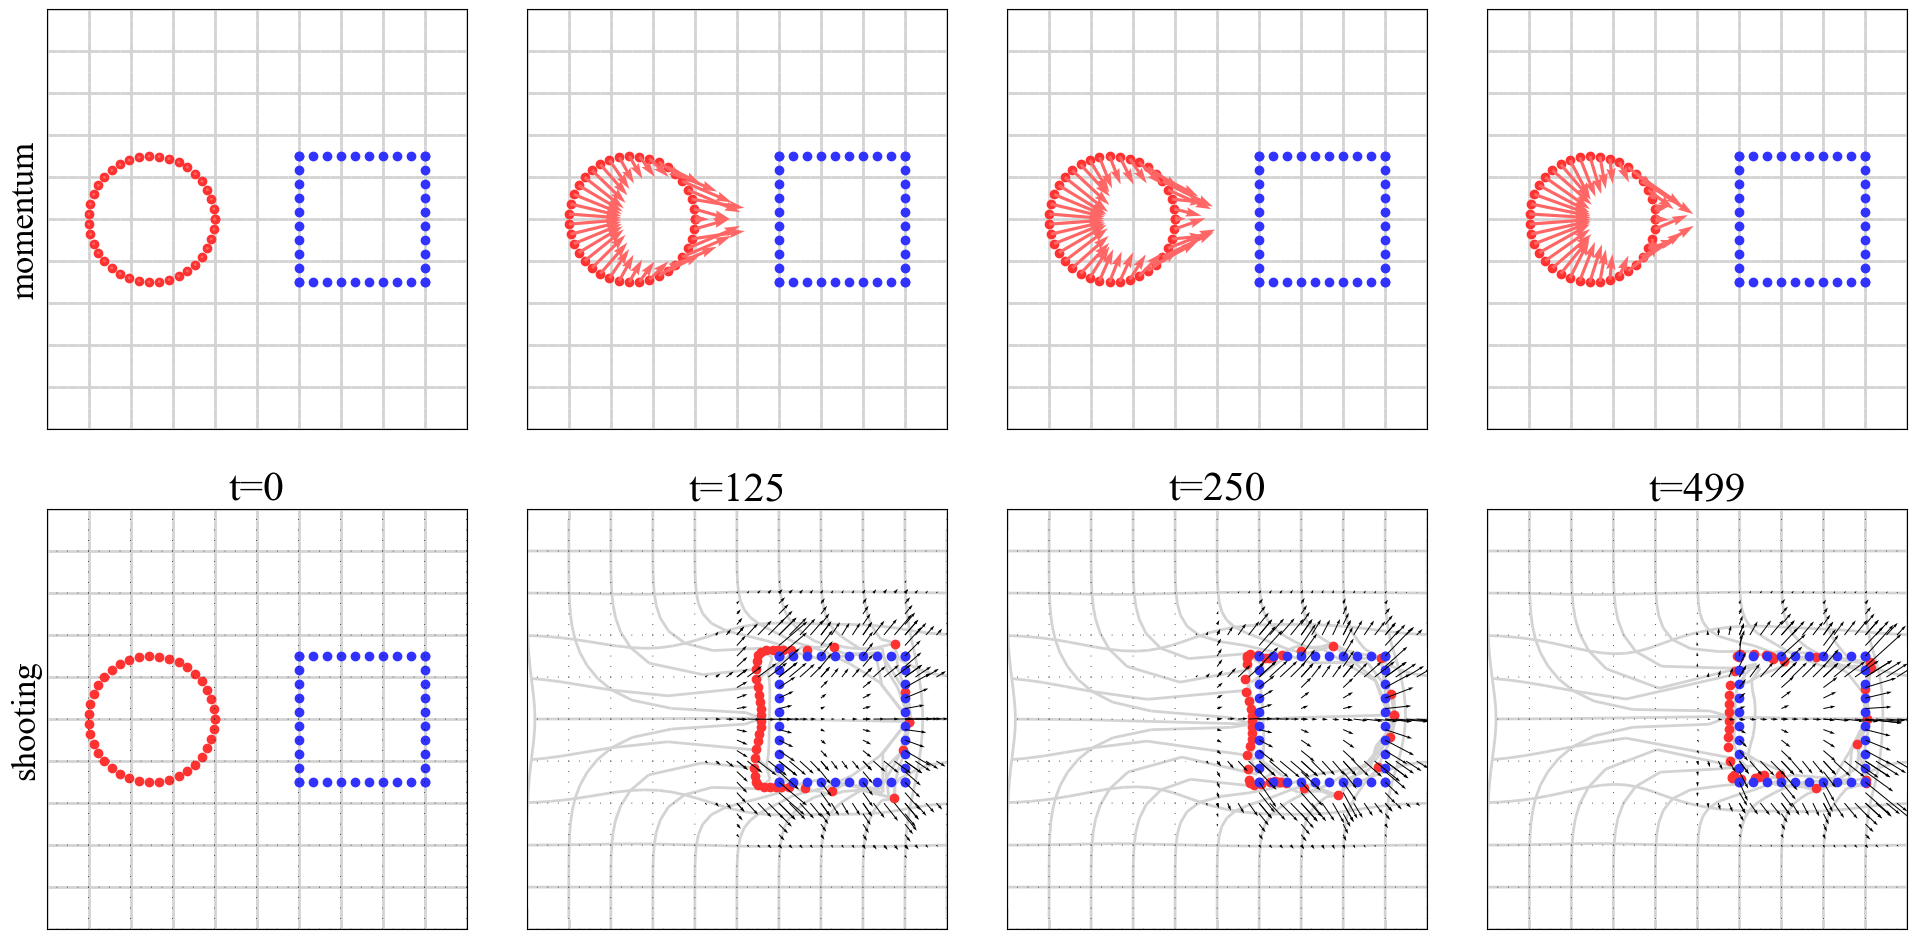
\includegraphics[width=\linewidth]{assets/plt_shooting} 
    \caption{Geodesic shooting with an Euler integrator with time step of $\delta t = .1$. The velocity field is represented using a radial basis kernel with $\sigma=.25$. We show trajectory of $q_t$ (red dots) with momentum $p_t$ (blue arrow) and interpolated velocity fields at grid points (black). We see Hamiltonian is approximately conserved!}
    \label{fig:plt_shooting}
\end{figure} 
\end{center}

% $\alpha,\beta$ is not restricted to probability measures 

\subsection{Unbalanced Regularized Optimal Transport}

Define $c:\Omega^2 \to \R$ be cost of mass transportation, hereafter we let $c$ be the squared Euclidean distance. The entropic regularized unbalanced optimal transport problem seeks a soft coupling between measures $\mu,\nu$ supported over $\Omega$ that minimizes expected cost; The optimal value of which defines a measure of similarity between $\mu$ and $\nu$,
\begin{align}
    \sW_{\epsilon,\rho}(\mu,\nu)
        := \min_{\pi\in\sP(\Omega^2)}\,
            \iint_{\Omega^2} c(x,y)\, d\pi(x,y) + \epsilon \text{KL}(\pi \Vert \mu\otimes\nu) \\
                \quad\quad+\rho\left( \text{KL}(P^1_\sharp \pi \Vert \mu) + \text{KL}(P^2_\sharp \pi \Vert \nu) \right)
    \label{eq:ot_wasserstein_regularized_unbalanced}
\end{align}
$P^i_\sharp$ is the projection to the $i$-th marginal. The correspondence of the optimal transport plan $\pi$ can be made sharper by using a smaller $\epsilon >0$. If the two shapes vary in scale, we can relax the mass conservation constraints by using a smaller $\rho>0$. 

For discrete measures, generalized Sinkhorn's algorithm computes $W_{\epsilon,\rho}(\alpha,\beta)$ efficiently and in a numerically stable manner \cite{chizatScalingAlgorithmsUnbalanced2017,feydyInterpolatingOptimalTransport2018}. The idea is to do coordinate ascent over the dual variables $u\in\R^N,v\in\R^M$,
\begin{align}
    u^{(\ell+1)}
        &\leftarrow \frac{\epsilon\rho}{\rho+\epsilon} \left( \log(a) - \log(Ke^{v^{(\ell)}/\epsilon}) \right) \\
    v^{(\ell+1)}
        &\leftarrow \frac{\epsilon\rho}{\rho+\epsilon} \left( \log(b) - \log(Ke^{u^{(\ell+1)}/\epsilon}) \right)
    \label{eq:sinkhorn_dual_ascent}
\end{align}
where $K\in\R^{N\times M}$ defined as $\pb{K}_{ij} = e^{-c(x_i,y_j)/\epsilon}$ is the Gibbs kernel. This algorithm, unlike the original matrix scaling algorithm, is numerically stable due to computation in log domain. A desirable property of optimal transport problem is that gradients of $W_{\epsilon,\rho}(\alpha,\beta)$ with respect to $x_i,a_i$ is readily computable, prompting easy integration into existing gradient based methods for registration problems \cite{feydyOptimalTransportDiffeomorphic2017a}. 


\section{Technical Approach}\label{sec:technical_approach}

\subsection{Registration as MAP Inference}

Diffeomorphic registration with geodesic shooting can be treated as a maximum a posteriori problem of initial velocity fields $v$ with a fixed Guassian process prior $v \sim \sG\sP(0,k)$ and a likelihood specified by the data matching term $\sW_{\epsilon,\rho}$,
\begin{align}
    P(v\mid x)
        &\propto \exp(-\frac{1}{2} x^TK(x,x)^{-1}x) \\
    P(y\mid x, v)
        &\propto \exp(-\sW_{\epsilon,\rho}(\varphi_\sharp \alpha, \beta))
    \label{eq:registration_prior_and_likelihood}
\end{align}
maximization of log posterior $\max_v \log P(v\mid x,y)$ recovers (\ref{eq:optimization_lddmm_landmark_momentum}). Suppose we obtained the optimal plan $\pi^*$, the likelihood is an isotropic multivariate normal over a weighted combination of $y$ centered at $q_1$ with variance determined by $\pi^*$.
\begin{align}
    \sW_{\epsilon,\rho}(\varphi_\sharp\alpha,\beta)
        &= \sum_{i=1}^N \sum_{j=1}^M \norm{q_1^i - y^j}_2^2 \pi_{ij}^* + \text{const} \\
        &= \sum_{i=1}^N \frac{1}{\sigma^2_i} \norm{q_1^i - \overline{y}^i}_2^2 + \text{const} \\
        &= (\overline{y} - q_1)^T \Sigma^{-1} (\overline{y} - q_1) + \text{const}
\end{align}
where $\sigma_i^2 = 1/(\sum_{j}\pi_{ij}^*)$, $\Sigma = \diag(\sigma_1^2,\cdots,\sigma_N^2)\otimes I_D$ are variances and $\overline{y}_i = \sum_j \sigma_i \pi_{ij}^* y^j$ is a weighted combination of $y$ with weights summing to 1, which we group together as $\overline{y} = (\overline{y}^1,\cdots,\overline{y}^N) \in \R^{ND}$. Intuitively, $q_1^i$ is matched with $\overline{y}^i$ by the transport plan, albeit at a synthetic location. The likelihood of observing $\overline{y}^i$ is large if it is close to $q_1^i$ and if the total mass coming from $q_1^i$, i.e. $\sum_{j}\pi_{ij}^*$, is small, indicating a larger uncertainty as to where transport plan might assign the point to. 

Of course, the behavior of the transport plan is affected by $\epsilon,\rho$. This might suggest inclusion of hyperparameters $\epsilon,\rho$ as optimziation variables of the likelihood model, akin to how we might want to optimize for the variance of an iid Gaussian noise model for registering images.

\subsection{Variational Inference with Average Transport Cost}

Let $y$ be observed variables, initial velocity field $v$ as latent variables. We are interested in the posterior density, $P(v\mid x, y) \propto P(v\mid x) P(y\mid v,x)$ where prior and likelihood is as defined in (\ref{eq:registration_prior_and_likelihood}). We define variational distribution over velocity vector field $Q(v)$ as a linear function of a free-form initial momentum $p_0$ with density $Q(p_0)$ via (\ref{eq:eulerian_velocity_interpolation}). We parameterize the initial momentum instead of velocity because we do not need to invert the kernel matrix $K(x,x)$ whenever we want to generate random diffeomorphic maps at test time. 

Let $\theta$ be the set of variational parameters to be optimized, encompassing parameters for $Q(p_0)$ and hyperparameter of kernel $k$. Inference relegates to finding an approximate posterior $Q(v)$ that is close to the true posterior using optimization, $\min_{\theta} \text{KL}(Q(v)\Vert P(v\mid x, y))$. As usually done in variational inference, we optimize the \text{ELBO},
\begin{align}
    \min_{\theta}\,
        \text{KL}(Q(v\mid x)\Vert P(v\mid x)) + \int \sW_{\epsilon,\rho}(\varphi_\sharp\alpha,\beta) \, dQ(p_0)
    \label{eq:opt_elbo1}
\end{align}
The second term can be approximated via Monte Carlo integration, but will be computationally inefficient due to need to solve several discrete transport problems for each gradient update to $\theta$. Alternatively, we optimize an upper bound, requiring one solve with a modified transport cost $\widetilde{c}: \Omega^2\to\R$ that marginalizes over $p_0$,
\begin{align}
    \widetilde{c}(x,y)
        = \int c(q_1(x,p_0),y)\, dQ(p_0)
    \label{eq:cost_marginalize_momentum}
\end{align}
Notationally, $q_1(p_0,\alpha)$ emphasizes the fact that $q_1$ is a deterministic function of $(p_0,\alpha)$ via (\ref{eq:geodesic_equations}). So,
\begin{align}
    \int \text{OT}^c(\varphi_\sharp\alpha,\beta) \, dQ(p_0)
        &\leq \text{OT}^{\widetilde{c}}(\alpha,\beta) \\
    \text{with}\quad \text{OT}^c(\alpha,\beta)
        &= \min_{\pi\in\Pi(\alpha,\beta)} \iint_{\Omega^2} c(x, y) \, d\pi(x,y)
\end{align}
This relationship also holds for regularized unbalanced cost. It is interesting that we are essentially computing optimal transport on source and target shapes directly, and that the randomness in $\varphi$ is incoporated into $\widetilde{c}$. Employing this upper bound for optimization of (\ref{eq:opt_elbo1}), we arrive at an objective that is computationally more tractable with the risk of derailing the optimization from good solutions.
\begin{align}
    \min_{\theta}\,
        \text{KL}(Q(v\mid x)\Vert P(v\mid x)) + \sW_{\epsilon,\rho}^{\widetilde{c}}(\alpha,\beta)
    \label{eq:opt_elbo2}
\end{align}


\subsection{Registration Uncertainty}

We can visualize the marginal variance of $Q(v)$ as well as a measure of spread of transformed points to get a sense of behavior of registration. There is no analytic formula for $\text{var}(q_1)$, and so we estimate it via $L$ samples,
\begin{align}
    \widehat{var}(q_1)
        &= \frac{1}{L} \sum_{l=1}^L (q_1^l-\widehat{\mu}(q_1)) (q_1^l-\widehat{\mu}(q_1))^T \\
    \widehat{\mu}(q_1)
        &= \frac{1}{L} \sum_{l=1}^L q_1^l 
    \quad\text{where}\quad
        q_1^l = q_1(g, p_0^l),\;\;
        p_0^l \overset{iid}{\sim} Q(p_0)
\end{align}
where $g\in\Omega^J$ is some gridded locations. We compute $\tr(\widehat{var}(q_1))$ as a scalar measure of uncertainty. The latter is often more informative, and correlates qualitatively to locations where the points are transported incorrectly, see~Figure (\ref{fig:plt_two_types_of_uncertainty}).

\begin{figure}[h!]
    \begin{center} 
    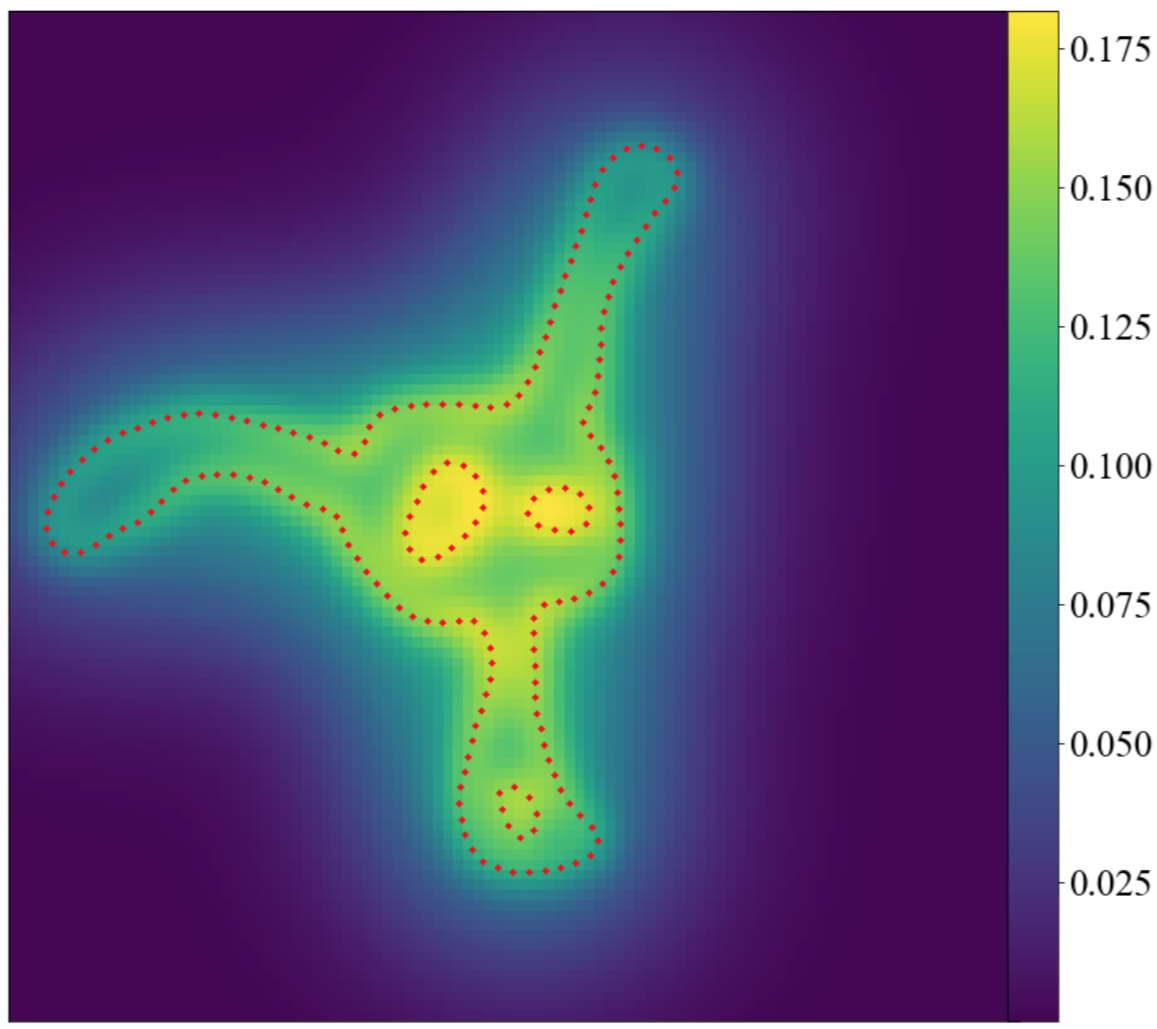
\includegraphics[width=.43\linewidth]{{assets/amoeba0/variance_velocity}}
    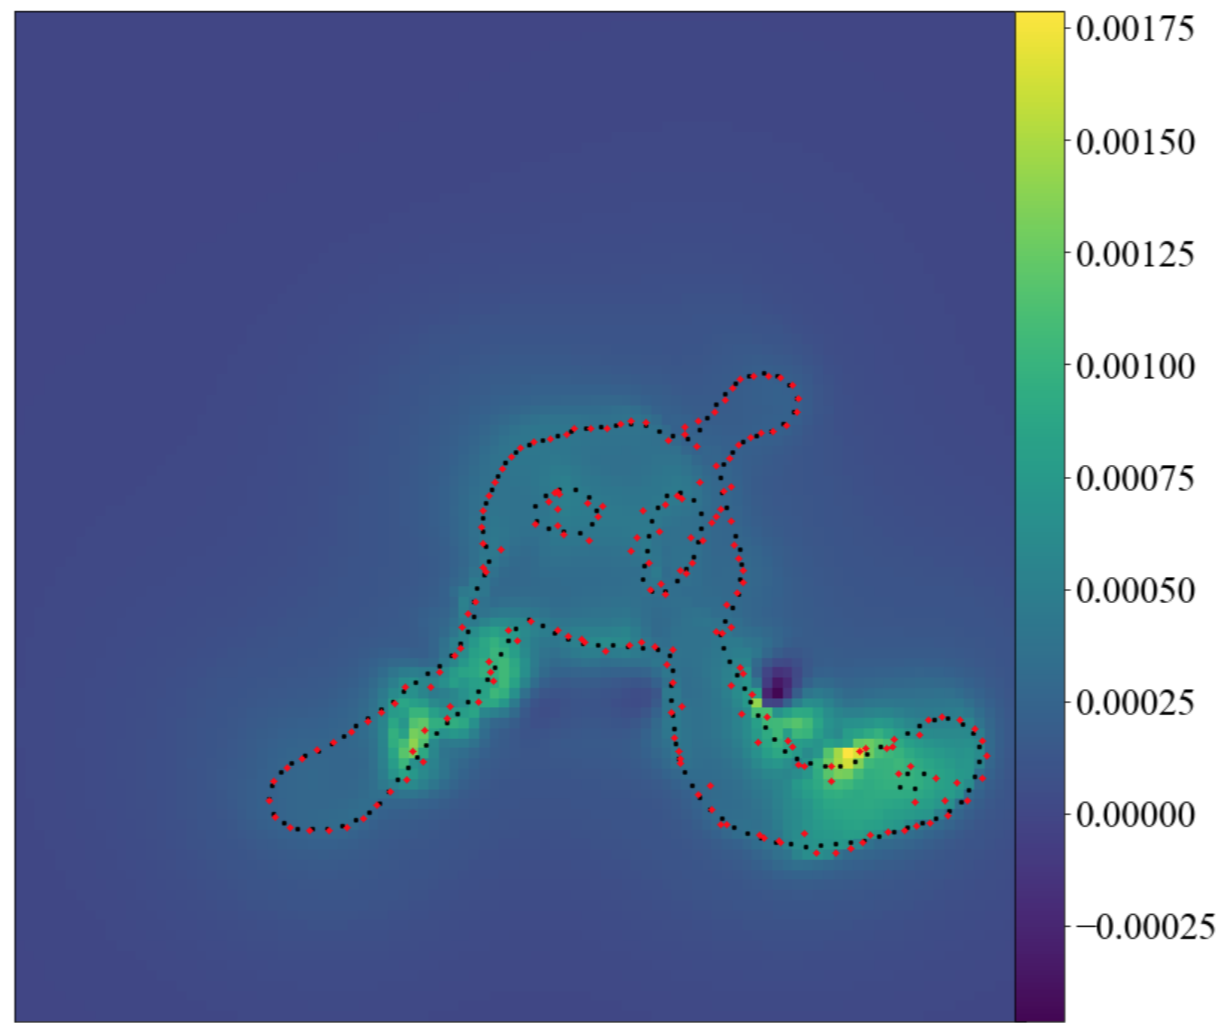
\includegraphics[width=.45\linewidth]{{assets/amoeba0/variance_q1}}
    \caption{(left) velocity marginal variance $\sigma^2(Q(v))$ (right) measure of spread of transformed points $\tr(\widehat{var}(q_1))$}
    \label{fig:plt_two_types_of_uncertainty}
\end{center}
\end{figure} 


\begin{figure*}[t]
    \begin{center} 
    \includegraphics[width=\linewidth]{{assets/shapes/plt_lddmm_points}}
    \includegraphics[width=\linewidth]{{assets/bat/plt_lddmm_points}}
    \caption{(left) two segmented shapes (middle right) estimated initial momentum (middle right) shape transformation (right) $\tr(\widehat{var}(q_1))$}
    \label{fig:plt_visualize_correct}
\end{center}
\end{figure*} 



\begin{figure*}[t]
    \begin{center} 
    \includegraphics[width=\linewidth]{{assets/amoeba0/plt_lddmm_points}}
    \includegraphics[width=\linewidth]{{assets/deer/plt_lddmm_points}}
    \caption{(left) two segmented shapes (middle right) estimated initial momentum (middle right) shape transformation (right) $\tr(\widehat{var}(q_1))$}
    \label{fig:plt_visualize_error}
\end{center}
\end{figure*} 

\section{Results}


\subsection{Dataset}

We used synthetic shape (amoeba) from \cite{feydyOptimalTransportDiffeomorphic2017a}. To re-iterate, the target is synthetically generated using a sum of Gaussian kernels with output variance $\pc{1., .75}$ and input standard deviation of $\pc{.025, .15}$.

In addition, take some images from MPEG7, a dataset of binary images for shape retrieval applications. We segment the shape via a simple thresholding on the image values and parameterize the shape with curves.

\subsection{Implementation}

For simplicity, we use a simple isotropic multivariate normal for $Q(p_0)$ with equal variance at each location $x\in\Omega$. the variational distribution for $v$ is also a multivariate normal via (\ref{eq:eulerian_velocity_interpolation}),
\begin{align}
    Q(p_0)
        &= \sN(p_0\mid \mu, \diag(w) \otimes I_D) \\
    Q(v\mid x)
        &= \sN(v\mid K(x,x)\mu, K(x,x) (\diag(w)\otimes I_D) K(x,x)^T)
\end{align}
We use radial basis kernel $k(x,y) = \sigma^2 \exp(-\norm{x-y}_2^2/\ell^2)$ with hyperparameter $\sigma^2,\ell$. In summary, $\theta = \pc{\mu,w,\sigma^2,\ell}$.

We approximate the cost matrix $\widetilde{C}_{ij}=\widetilde{c}(x_i,y_j)$ via sampling, i.e. sample random trajectories, compute pairwise cost between transformed and target shapes, and then averaging the costs. We simply use gradient descent to optimize for (\ref{eq:opt_elbo2}). 

We optimize for hyperparameters through an adaptive gradient method, e.g. ADAM. The gradient of the KL term requires $\sO((ND)^3)$ computation and $\sO((ND)^2)$ memory due to need for a Cholesky factorization, a significant addition to compute cost from previous methods that computes the MAP solution. To reduce cost to $\sO(N^3)$ computation and $\sO(N^2)$ memory, we assume that the kernel is the same regardless of $d=1,\cdots,D$, i.e. $K=K'\otimes I_D$ for some $K'\in\R^{n\times n}$. The cost for computing gradients $\nabla_{\theta} \sW_{\epsilon,\rho}^{\widetilde{c}}(\alpha,\beta)$ is primarily dominated by ODE solves and Sinkhorn's iterations. We keep a fixed 10 samples to approximate $\widetilde{C}$ and a fixed 100 iterations to solve for the optimal transport problem. We have experimented with as little as 1 samples for approximating $\widetilde{C}$, but the variance of gradient is too large for the optimization to converge to a reasonable local minima. For simplicity, we just autodiff to accumulate gradient through Sinkhorn's iteration as \cite{genevayLearningGenerativeModels2018} instead of computing gradients of OT cost with respect to the optimal transport plan. We backprop through sampling of $p_0$ using reparamterization trick originally proposed for training variational autoencoders.

We fix $\epsilon=.15^2$ and pick $\rho$ such that $\epsilon\rho/(\rho+\epsilon) = .998$. We also weight the KL term in the loss functions with constant $\lambda = .003$.

When estimating registration uncertainty, we set $L=100$ and interpolate via thin-plate spline to obtain a smooth heat map.


\subsection{Registration Errors}

We want to visualize uncertainty of transformed shape. For shapes that are correctly registered, we notice that similar levels of uncertainty is located on the boundary of the curve, as shown in Figure~\ref{fig:plt_visualize_correct}. On the contrary, for shapes that are not correctly registered, due to some complicated nonlinear deformations, we see higher uncertainty in regions where shapes are incorrectly matched in Figure~(\ref{fig:plt_visualize_error})


\newpage
\newpage

\bibliographystyle{eg-alpha-doi}
\bibliography{optimal_transport,registration,GP}


\end{document}
